%------------------------------------------------------------------------------------
%	CHAPTER 3
%------------------------------------------------------------------------------------
\chapterimage{headSpark.png}
\chapter{Aprofundando no Spark}

\begin{remark}
"Uma única centelha de criatividade pode desencadear uma revolução tecnológica e transformar o mundo." (Elon Musk) 
\end{remark}

\section{Melhora dos Dados Estatísticos}\index{Aprofundando no Spark}
\textbf{Ming Chen} e \textbf{Wenqiang Feng} escreveram um excelente método que se compara bem ao método describe() da biblioteca Pandas (com algumas vantagens), sendo assim, vamos aplicá-la. Criamos um novo notebook e em uma célula a conexão com o Spark:
\begin{lstlisting}[]
from pyspark.sql import SparkSession

spark = SparkSession.\
        builder.\
        appName("pyspark-notebook").\
        master("spark://spark-master:7077").\
        config("spark.executor.memory", "512m").\
        getOrCreate()
\end{lstlisting}

Em seguida criamos um Dataframe:
\begin{lstlisting}[]
df_pyspark = spark.read.csv('dados2.csv', header=True, inferSchema=True)
df_pyspark.show()
\end{lstlisting}

Lembre-se que o arquivo se encontra disponível no GitHub, usamos o método describe nativo:
\begin{lstlisting}[]
df_pyspark.describe().show()
\end{lstlisting}

E temos o seguinte resultado:
 \vspace{-1.5em}
\begin{verbatim}
+-------+---------+------------------+------------------+
|summary|     Nome|             Idade|       Experiencia|
+-------+---------+------------------+------------------+
|  count|       54|                54|                54|
|   mean|     null| 44.96296296296296|107.57407407407408|
| stddev|     null|15.026973185930618| 86.78679185044531|
|    min|    Alice|                18|                 0|
|    max|Valentina|                73|               444|
+-------+---------+------------------+------------------+
\end{verbatim}

Agora precisamos usar o Pandas, apenas para organizar melhor a informação:
\begin{lstlisting}[]
!pip install pandas
\end{lstlisting}

Uma vez instalado, podemos realizar as importações necessárias para execução do método:
\begin{lstlisting}[]
import numpy as np
import pandas as pd
\end{lstlisting}

E criar o método:
\begin{lstlisting}[]
def describe_pd(df_in, columns, deciles=False):
    if deciles:
        percentiles = np.array(range(0, 110, 10))
    else:
        percentiles = [25, 50, 75]
    percs = np.transpose([np.percentile(df_in.select(x).collect(),percentiles) for x in columns])
    percs = pd.DataFrame(percs, columns=columns)
    percs['summary'] = [str(p) + '%' for p in percentiles]
    spark_describe = df_in.describe().toPandas()
    new_df = pd.concat([spark_describe, percs],ignore_index=True)
    new_df = new_df.round(2)
    return new_df[['summary'] + columns]
\end{lstlisting}

Esse método pode ser trabalhado tanto com deciles quanto os percentis, para usar os deciles basta usar o parâmetro "deciles=True", por padrão a saída é dada em percentis, porém só podemos usar as colunas numéricas, do seguinte modo:
\begin{lstlisting}[]
describe_pd(df_pyspark, ['Idade', 'Experiencia'])
\end{lstlisting}

E temos como resultado:
\begin{figure}[H]
	\centering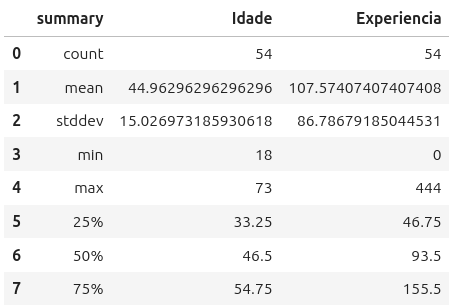
\includegraphics[scale=0.45]{cap03/SaidaDescribe}
	\caption{Saída do método describe\_pd()}
\end{figure}

E deste modo obtemos um visual bem mais agradável.

\section{Assimetria e Curtose}\index{Aprofundando no Spark}

Na probabilidade, \textbf{assimetria} (ou \textit{skewness} em inglês) é uma medida de assimetria da distribuição de probabilidade em uma variável aleatória com valores reais em relação à sua média. O valor de assimetria pode ser positivo, negativo ou indefinido. Para uma distribuição unimodal, uma assimetria negativa indica comumente que a cauda está do lado esquerdo da distribuição, enquanto uma assimetria positiva indica que a cauda está do lado direito.

Já a palavra, \textbf{curtose} (ou \textit{kurtosis} em inglês, também escrito como "kyrtos" ou "kurtos", significando "curvado, arqueado") é uma medida de "caudalidade" da distribuição de probabilidade em uma variável aleatória com valores reais. De maneira similar ao conceito de assimetria, a curtose é um descritor da forma em uma distribuição de probabilidade e, assim como para a assimetria, existem diferentes maneiras de quantificá-la para uma distribuição teórica e métodos correspondentes para estimá-la a partir da amostra de uma população.

Importamos as bibliotecas necessárias:
\begin{lstlisting}[]
from pyspark.sql.functions import col, skewness, kurtosis
\end{lstlisting}

E executamos os métodos para a variável idade:
\begin{lstlisting}[]
df_pyspark.select(skewness(df_pyspark.Idade),kurtosis(df_pyspark.Idade)).show()
\end{lstlisting}

E temos o seguinte resultado:
 \vspace{-1.5em}
\begin{verbatim}
+-------------------+-------------------+
|    skewness(Idade)|    kurtosis(Idade)|
+-------------------+-------------------+
|0.08635507023568641|-0.9555352263232475|
+-------------------+-------------------+
\end{verbatim}

Uma assimetria positiva indica que a cauda direita é mais longa, se fosse uma assimetria negativa a cauda esquerda seria mais longa, em relação a um centro típico dos dados. Vejamos isso graficamente, porém precisamos instalar a biblioteca SeaBorn:
\begin{lstlisting}[]
!pip install seaborn
\end{lstlisting}

Uma vez instalada, podemos importar as bibliotecas necessárias:
\begin{lstlisting}[]
\textbf{import seaborn as sns
import matplotlib.pyplot as plt
%matplotlib inline}
\end{lstlisting}

Obter os valores que serão mostrados:
\begin{lstlisting}[]
coluna_selecionada = df_pyspark.select("Idade")
x = coluna_selecionada.rdd.flatMap(lambda x: x).collect()
\end{lstlisting}

E mostrar o gráfico:
\begin{lstlisting}[]
plt.figure(figsize=(8,4))
sns.histplot(x, kde=True)
plt.xlabel('Idade')
plt.ylabel('Quantidade')
plt.show()
\end{lstlisting}

E temos como resultado:
\begin{figure}[H]
	\centering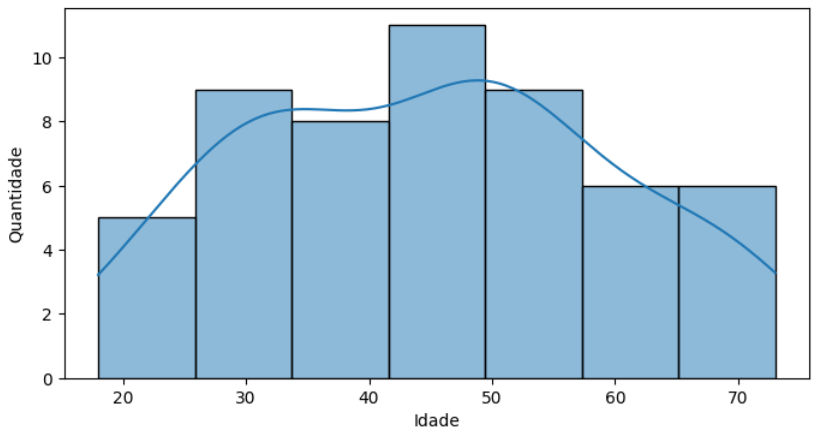
\includegraphics[scale=0.45]{cap03/GraficoDistribuicao}
	\caption{Gráfico da Distribuição por Idade}
\end{figure}

\section{Métodos Estatísticos com RDD}\index{Aprofundando no Spark}
Objetos RDD são interessantes quando desejamos informações básicas estatísticas, nesta seção veremos uma série de exemplos, inicialmente criamos um novo notebook e iniciamos a seção do Spark neste:
\begin{lstlisting}[]
from pyspark.sql import SparkSession

spark = SparkSession.\
        builder.\
        appName("pyspark-notebook").\
        master("spark://spark-master:7077").\
        config("spark.executor.memory", "512m").\
        getOrCreate()
        
sc = spark.sparkContext        
\end{lstlisting}

Criamos nossos dados através da paralelização de uma lista de valores:
\begin{lstlisting}[]
numsRdd = sc.parallelize((2, 4, 6, 8, 3, 2, 8, 1, 4, 7))
\end{lstlisting}

A média aritmética desses valores:
\begin{lstlisting}[]
numsRdd.mean()
\end{lstlisting}

E obtemos o valor: \\
{\ttfamily 4.5}

A quantidade de elementos (ou amostras):
\begin{lstlisting}[]
numsRdd.count()
\end{lstlisting}

E obtemos o valor: \\
{\ttfamily 10}

Quantidade de cada um dos valores:
\begin{lstlisting}[]
numsRdd.countByValue()
\end{lstlisting}

E obtemos o valor: \\
{\ttfamily defaultdict(int, \{2: 2, 4: 2, 6: 1, 8: 2, 3: 1, 1: 1, 7: 1\})}

O primeiro valor da lista:
\begin{lstlisting}[]
numsRdd.first()
\end{lstlisting}

E obtemos o valor: \\
{\ttfamily 2}

O maior e menor valor da lista
\begin{lstlisting}[]
print(numsRdd.max(), numsRdd.min())
\end{lstlisting}

E obtemos os valores: \\
{\ttfamily 8 1}

Desvio padrão:
\begin{lstlisting}[]
numsRdd.stdev()
\end{lstlisting}

E obtemos o valor: \\
{\ttfamily 2.4596747752497685}

A soma total dos valores:
\begin{lstlisting}[]
numsRdd.sum()
\end{lstlisting}

E obtemos o valor: \\
{\ttfamily 45}

Também podemos usar o método de agregação \textit{fold()} que reúne os elementos do RDD através um valor neutro especificado (valor zero) e um operador binário associativo. Primeiro agrega os elementos em cada partição do RDD e, em seguida, agrega os resultados de cada partição:
\begin{lstlisting}[]
# Soma de todos os elementos do RDD
soma = numbersRdd.fold(0, lambda x, y: x + y)

# Produto de todos os elementos do RDD
produto = numbersRdd.fold(1, lambda x, y: x * y)
print(soma, produto)
\end{lstlisting}

E obtemos os valores: \\
{\ttfamily 45 516096}

Neste exemplo, o método fold() recebe dois argumentos: o primeiro é o valor inicial (0 para a soma e 1 para o produto) e o segundo é a função lambda que combina os elementos do RDD (soma ou multiplicação) de acordo com a operação desejada.

Porém é mais eficiente utilizarmos o método reduce() que agrega os elementos do RDD usando um operador binário associativo e comutativo fornecido. É semelhante ao método fold(); no entanto, não requer um valor neutro:
\begin{lstlisting}[]
# Soma de todos os elementos do RDD
soma = numbersRdd.reduce(lambda x, y: x + y)

# Produto de todos os elementos do RDD
produto = numbersRdd.reduce(lambda x, y: x * y)
print(soma, produto)
\end{lstlisting}

E teremos o mesmo resultado, a diferença é que o método reduce() recebe somente a função lambda com dois argumentos (x e y), representando dois elementos do RDD que serão combinados para calcular o resultado final. 

E a variância:
\begin{lstlisting}[]
numsRdd.variance()
\end{lstlisting}

E obtemos o valor: \\
{\ttfamily 6.05}

Não esquecer de encerrar a seção:
\begin{lstlisting}[]
spark.sparkContext.stop()
\end{lstlisting}

\clearpage